\capitulo{5}{Resultados}

\section{Resumen de resultados}

Como ya se ha comentado previamente en los apartados de ``Objetivos'' y ``Metodología'', en este trabajo se han realizado diversas comparaciones con el fin de encontrar el mejor modelo de red neuronal acorde a nuestro caso, es decir, para determinar correctamente si existe o no neumonía a partir de un conjunto de imágenes médicas de CXT.

Hay que tener en cuenta que, cada vez que se ejecuta el código de Python realizado para la obtención de predicciones de imágenes a partir de redes neuronales, los resultados pueden variar sutilmente debido principalmente a:
\begin{itemize}
    \item El valor de los pesos iniciales (w) se asignan de manera aleatoria. Por lo que, cada vez que se ejecuta el entrenamiento, los pesos iniciales pueden ser distintos, lo que lleva a resultados ligeramente diferentes en las predicciones.
    \item Las muestras de entrenamiento también se seleccionan de manera aleatoria por lo que, en cada ejecución el subconjunto de datos seleccionado para entrenar el modelo puede ser distinto, lo que hace variar ligeramente los resultados.
\end{itemize}

Por lo tanto, en cada ejecucion se parte de un estado diferente.

\subsection{Comparación entre arquitecturas y \textit{batch size} con CNN propia y CNN AlexNet}

En primer lugar, se ha realizado con Python una tabla comparativa entre tres modelos de arquitectura distintos (explicados en el apartado de ``Metodología'') y cuatro valores distintos de \textit{batch size} (8, 16, 20, 32, 64) tanto para la CNN propia como para la CNN AlexNet.

En dichas tablas, se han calculado diversas métricas para determinar cuál es el mejor modelo. Antes de comenzar a calcular las métricas, es necesario obtener la matriz de confusión para obtener los verdaderos positivos (TP), verdaderos negativos (TN), falsos positivos (FP) y falsos negativos (FN) y, a partir de estos valores se calculan las métricas.

\begin{figure}[h]
    \centering
    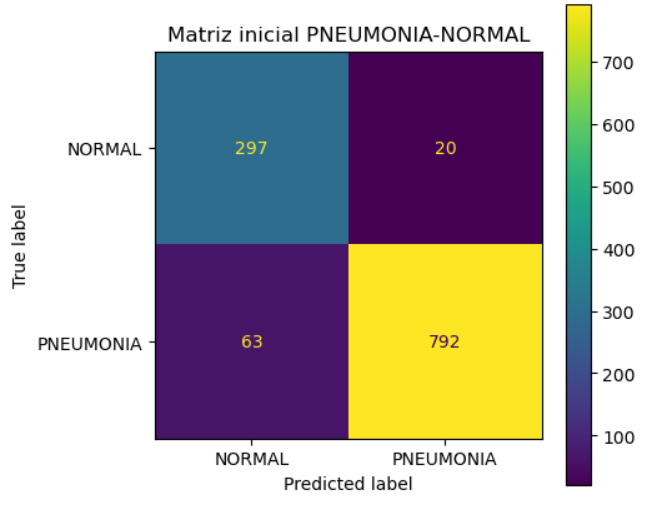
\includegraphics[width=0.80\textwidth]{img/matriz_conf_inicial.PNG}
    \caption{Matriz de confusión inicial. Fuente propia}
    \label{fig:matriz_confusion_inicial}
\end{figure}

\begin{itemize} 
    \item \textbf{Verdaderos positivos (TP)}: cantidad de positivos que fueron clasificados correctamente por el modelo como positivos. En la figura \ref{fig:matriz_confusion_inicial} se corresponde con los casos que el modelo predice como neumonía y realmente el paciente tiene neumonía (valor 792).
    \item \textbf{Verdaderos negativos (TN)}: cantidad de negativos que fueron clasificados correctamente por el modelo como negativos. En la figura \ref{fig:matriz_confusion_inicial} se corresponde con los casos que el modelo predice como normal y realmente el paciente no tiene neumonía (valor 297).
    \item \textbf{Falsos positivos (FP)}: cantidad de negativos que fueron clasificados incorrectamente por el modelo como positivos. En la figura \ref{fig:matriz_confusion_inicial} se corresponde con los casos que el modelo predice como neumonía pero realmente el paciente no tiene neumonía (valor 20).
    \item \textbf{Falsos negativos (FN)}: cantidad de positivos que fueron clasificados incorrectamente por el modelo como negativos. En la figura \ref{fig:matriz_confusion_inicial} se corresponde con los casos que el modelo predice como normal pero realmente el paciente tiene neumonía (valor 63).
\end{itemize}

Una vez obtenidos los TP, TN, FP y FN, se calculan las siguientes métricas:

\begin{itemize}
    \item \textbf{\textit{Loss}}: se emplea para evaluar cómo un modelo de aprendizaje automático se ajusta a los datos de entrenamiento.
    
    Para calcular el valor de \textit{loss} en Python, no se emplea una fórmula concreta dada su complejidad sino que, se calcula mediante la función \textit{model.evaluate} que proporciona la biblioteca keras.
    \item \textbf{\textit{Acuracy} (o exactitud)}: proporción de predicciones correctas. 
    \begin{equation*}
        \text{\textit{accuracy}} = \frac{\text{TP + TN}}{\text{TN + FP + FN + TP}}
    \end{equation*}
    \item \textbf{\textit{Precision}}: proporción de predicciones positivas correctas
    \begin{equation*}
        \text{\textit{precision}} = \frac{\text{TP}}{\text{TP + FP}}
    \end{equation*}
    \item \textbf{\textit{Recall} (o sensibilidad)}: proporción de positivos detectados
    \begin{equation*}
        \text{\textit{recall}} = \frac{\text{TP}}{\text{TP + FN}}
    \end{equation*}
    \item \textbf{F1}:  media armónica de precisión y exhaustividad para evaluar de una forma más equilibrada el rendimiento del modelo.
    \begin{equation*}
        \text{F1} = \frac{\text{2 * \textit{precision} * \textit{recall})}}{\text{\textit{precision}+\textit{recall}}}
    \end{equation*}
    \item \textbf{\textit{Specificity} (o especificidad)}: proporción de negativos detectados
    \begin{equation*}
        \text{\textit{specificity}} = \frac{\text{TN}}{\text{TN + FP}}
    \end{equation*}
    \item \textbf{fpr (o tasa de falsos positivos)}: proporción de negativos incorrectamente clasificadas como positivos, respecto al total de casos negativos reales.
    \begin{equation*}
        \text{fpr} = \frac{\text{FP}}{\text{FP + TN}}
    \end{equation*}
    \item \textbf{fnr (o tasa de falsos negativos)}: proporción de positivos incorrectamente clasificadas como negativos, respecto al total de casos positivos reales.
    \begin{equation*}
        \text{fnr} = \frac{\text{FN}}{\text{FN + TP}}
    \end{equation*}
    \item \textbf{AUC (o área bajo la curva ROC)}: se emplea para evaluar la capacidad de distinción entre clases positivas y negativas de un modelo de clasificación binaria. Un 1 significa que es capaz de distinguir perfectamente entre clases, un 0.5 significa una clasificación aleatoria y un 0 indica que ninguna clase ha sido correctamente clasificada. Esto se puede ver mejor en la figura \ref{fig:roc}.
    \begin{figure}[h]
        \centering
        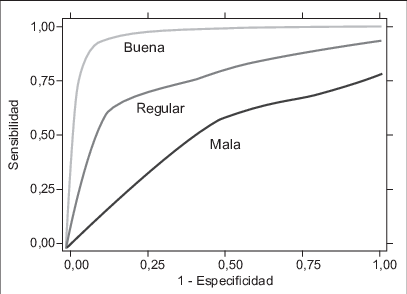
\includegraphics[width=0.70\textwidth]{img/roc.png}
        \caption{Ilustración tipos de curvas ROC. ~\cite{ResearchGate24}}
        \label{fig:roc}
    \end{figure}
    
    Para calcular el valor de AUC en Python, no se emplea una fórmula concreta dada su complejidad, sino que, se calcula mediante la función \textit{roc\_auc\_score} del módulo sklearn.
    
\end{itemize}

Una vez se han obtenido todos estos parámetros para cada una de las arquitecturas y cada uno de los valores de \textit{batch size} se comparan y se determina, cuál de las dos CNN funciona mejor y, una vez se tiene esto, se decide cual es la mejor arquitectura y, para esa arquitectura concreta se determina cual es el mejor valor de \textit{batch size}. Hay que tener en cuenta que, la mejor arquitectura es aquella con un valor mayor en todas las métricas (excepto \textit{loss}, fpr y fnr que interesa un valor menor).

\begin{figure}[h]
    \centering
    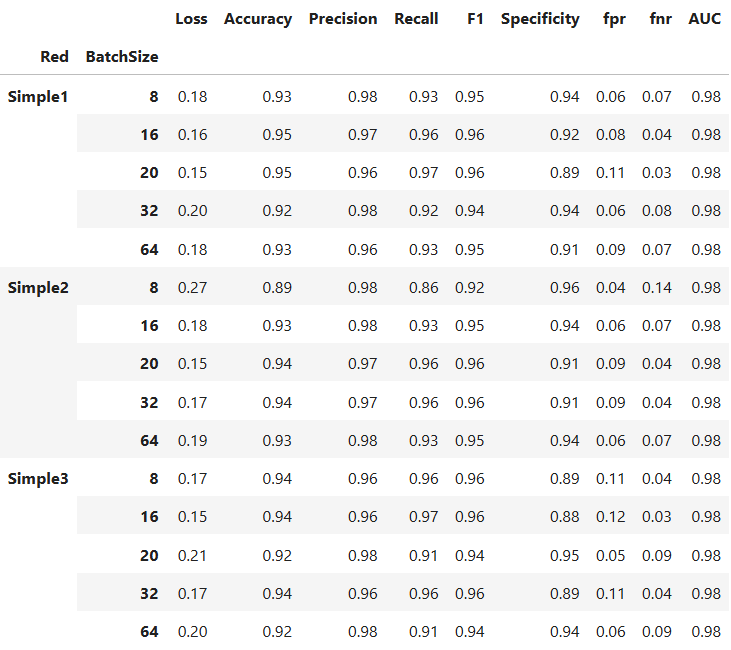
\includegraphics[width=0.99\textwidth]{img/tabla_propia_arqu_batch.PNG}
    \caption{Tabla comparativa de las distintas arquitecturas y \textit{batch size} con CNN propia. Fuente propia.}
    \label{fig:tabla_propia_arqu_batch}
\end{figure}
\FloatBarrier


\begin{figure}[h]
    \centering
    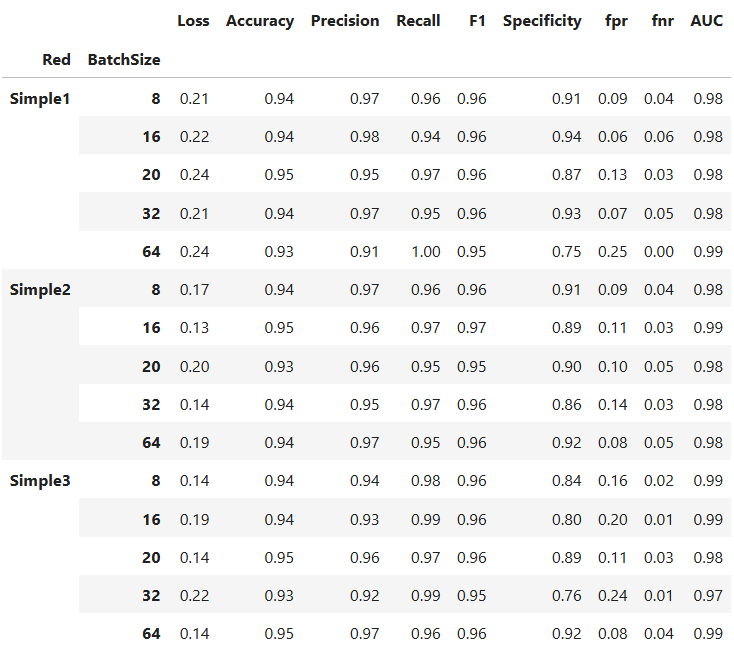
\includegraphics[width=0.99\textwidth]{img/tabla_alexNet_arqu_batch.PNG}
    \caption{Tabla comparativa de las distintas arquitecturas y \textit{batch size} con CNN AlexNet. Fuente propia.}
    \label{fig:tabla_alexNet_arqu_batch}
\end{figure}
\FloatBarrier

Previo a dictaminar los mejores resultados obtenidos en este caso, hay que tener en cuenta la aleatoriedad de pesos y muestras iniciales mencionados previamente, por lo que se obtienen resultados ligeramente distintos en cada ejecución. Debido a esto y a la similitud en los resultados obtenidos, se ha comprobado como cada vez que se ejecutaba se obtenían los mejores resultados en un modelo o en otro (excluyendo el modelo ``Simple1'' debido a su simplicidad). Por lo que, a continuación, se va a determinar el mejor modelo obtenido en este caso (en la ejecución del \textit{notebook} ``redes neuronales - neumonia'').

En primer lugar, con las tablas obtenidas para la CNN propia \ref{fig:tabla_propia_arqu_batch} y la de AlexNet \ref{fig:tabla_alexNet_arqu_batch}, se puede observar como en la tabla referida a la CNN de AlexNet existen valores mayores de AUC (una métrica que puede resultar muy interesante en este caso debido al desbalanceo que existe entre casos y controles) ya que hay varios valores de 0,99 mientras que en la de CNN propia en ningún caso sube de 0,98. Por lo tanto, se puede descartar la CNN propia y, a partir de ahora se trabaja con la CNN de AlexNet.

Antes de identificar la arquitectura óptima, hay que tener en cuenta que, el modelo ``Simple1'' es demasiado básico. En consecuencia, los resultados que ofrece no son muy buenos ya que, carece de capas ocultas y su arquitectura es extremadamente simple. Por lo que ha sido la primera arquitectura en descartarse. Sin embargo, es de gran utilidad para comprobar lo mal que predice el modelo en un principio y como este evoluciona. 

Ya que, tal y como se muestra en la figura \ref{fig:matriz_confusion_inicial}, donde se visualiza la matriz de confusión del modelo más simple (``Simple1'') con la CNN propia, se observa como en el hipotético caso de que este modelo no se mejorara y fuera utilizado en la vida real, 63 pacientes con neumonía serían diagnosticados como normal y 20 pacientes sin neumonía serían diagnosticados con neumonía. Esto supone unas cifras demasiado altas y acarrearía graves consecuencias en el ámbito de la sanidad. Por ello es necesario mejorar este modelo.

Una vez descartada la primera arquitectura, se realiza una comparación entre la segunda (``Simple2'') y la tercera (``Simple3''). Observando la \ref{fig:tabla_alexNet_arqu_batch} se puede determinar que, aunque los resultados son similares para ambas arquitecturas, existen valores mayores de AUC en el modelo ``Simple3'' y, por ellos se escoge como la mejor arquitectura. Como ya se ha comentado en el apartado de ``Metodología'', el modelo "Simple3" se corresponde con un modelo que posee varias capas convolucionales (con las que se obtienen características importantes de las imágenes) seguidas de capas de MaxPooling2D para reducir la dimensionalidad. También hay una capa oculta de 100 neuronas, una segunda capa oculta de 16 neuronas y una capa densa.

Una vez escogida la arquitectura, se determina cual es el mejor \textit{batch size} para esta arquitectura. De nuevo, observando la tabla \ref{fig:tabla_alexNet_arqu_batch}, se puede ver como los valores más altos de AUC existen para un \textit{batch size} de 8, 16 y 64 y, teniendo en cuenta que un \textit{batch size} mayor entrena la red en menos tiempo ya que, el \textit{batch size} es un compromiso entre precisión y tiempo de entrenamiento, el mejor \textit{batch size} en este caso es el de 64.

Resumiendo, se puede determinar que, en esta primera comparación y con lo que se va a trabajar a partir de ahora es la \textbf{CNN de AlexNet}, el modelo \textbf{``Simple3''} con un \textbf{\textit{batch size} de 64}.

\subsection{Comparación número de neuronas}
Partiendo de la CNN de AlexNet con el modelo ``Simple3'' y un \textit{batch size} de 64, se comparan distintos valores de neuronas en la capa oculta para este modelo.

El modelo ``Simple3'' presenta dos capas ocultas con neuronas. En este caso, para probar los distintos valores de neuronas en las capas ocultas, se han empleado los mismos valores en ambas capas, aunque, también se podría haber hecho diferenciando valores entre una capa y otra. Por lo general, la primera capa tiene el mismo o más neuronas que la segunda, y así sucesivamente. Los valores empleados han sido potencias de 2 tales como 512, 1024 y 2048.

Se emplean las mismas métricas que en el caso anterior para decidir cuál es el mejor modelo. Lo ideal es que todas las métricas excepto ``\textit{loss}'', ``fpr'' y ``fnr'' tengan el mayor valor. 

\begin{figure}[h]
    \centering
    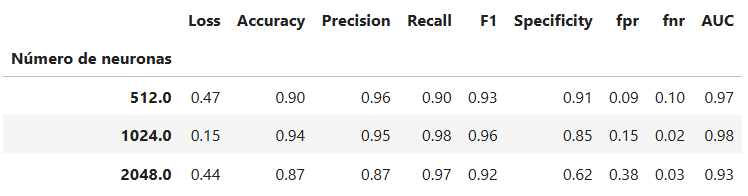
\includegraphics[width=0.99\textwidth]{img/tabla_num_neuronas.PNG}
    \caption{Tabla comparativa de distintos valores de neuronas en la capa oculta. Fuente propia.}
    \label{fig:tabla_num_neuronas}
\end{figure}
\FloatBarrier

Tal y como se puede observar en la tabla \ref{fig:tabla_num_neuronas}, comparando cada una de las métricas para los tres valores diferentes se puede ver que los resultados de las métricas son similares pero, fijándonos en el AUC, el mejor valor se encuentra para 1024 neuronas.

Aun así, comparando las métricas obtenidas para 1024 neuronas en las dos capas ocultas en comparación con las métricas de la tabla \ref{fig:tabla_alexNet_arqu_batch} en el modelo ``Simple3'', con un \textit{batch size} de 64 y 100 y 16 neuronas respectivamente en ambas capas ocultas (que son los valores que se han empleado en el modelo inicial) se puede concluir que, el mejor modelo se corresponde con la CNN de AlexNet, el modelo ``Simple3'', un \textit{batch size} de 64, y 100 y 16 neuronas en las capas ocultas respectivamente.

Con este modelo final se obtiene un AUC del 99\%, un \textit{accuracy} del 95\%, y una precisión del 97\% tal y como se puede observar en la figura \ref{fig:tabla_alexNet_arqu_batch}.

Para el modelo elegido finalmente, se ha obtenido tanto su matriz de confusión \ref{fig:matriz_conf_final} (para ser comparada con la matriz inicial \ref{fig:matriz_confusion_inicial}) como dos gráficas donde se representa el rendimiento del modelo a lo largo de tiempo en el entrenamiento y la validación respecto al AUC \ref{fig:grafica_auc_Simple3_64_100_16} y respecto a \textit{loss} \ref{fig:grafica_loss_Simple3_64_100_16}.  

\begin{figure}[h]
    \centering
    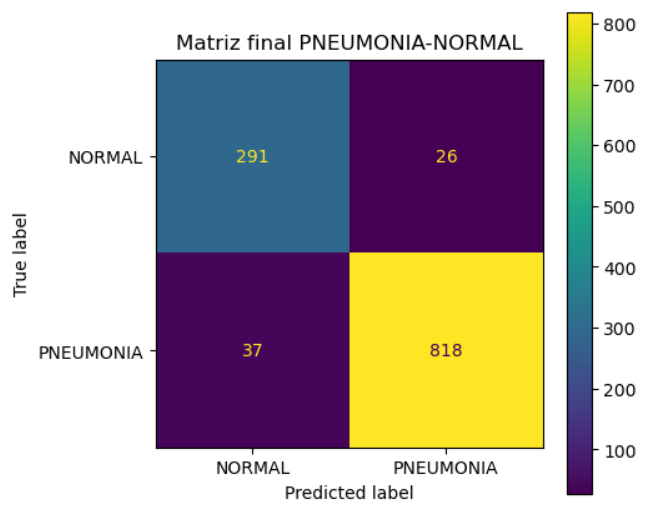
\includegraphics[width=0.80\textwidth]{img/matriz_conf_final.PNG}
    \caption{Matriz de confusión modelo final. Fuente propia.}
    \label{fig:matriz_conf_final}
\end{figure}

Con la matriz de confusión final \ref{fig:matriz_conf_final}, se puede apreciar cómo el valor de FP aumenta mientras que los FN disminuyen notablemente respecto a la matriz inicial. 

Tal y como se ha comentado al principio de este apartado, los FP se corresponden con aquellos pacientes sin neumonía diagnosticados por el modelo con neumonía y, los FN son aquellos que el modelo identifica como normal (o sano) pero en verdad se trata de un paciente con neumonía.

En el ámbito clínico, es preferible un modelo con un mayor número de FP que de FN ya que, los FP serán revisados más exhaustivamente por el personal clínico, quienes acabarán viendo que el paciente no tiene dicha enfermedad, por lo que no resulta en algo muy perjudicial para el paciente. Sin embargo, los FN, pueden ser mucho más peligrosos ya que, se diagnostica a un paciente como sano estando enfermo, lo que puede agravar la patología al no diagnosticarse a tiempo y causar daños irreparables para el paciente.

Por lo tanto, teniendo en cuenta esto último y comparando la matriz de confusión inicial \ref{fig:matriz_confusion_inicial} con la matriz de confusión final, \ref{fig:matriz_conf_final} se puede apreciar una mejora considerable ya que, aunque en la matriz de confusión final el valor de FP aumente, esto no es un problema serio en este caso. Además, el valor de FN disminuye notablemente, algo muy positivo a tener en cuenta debido a las consecuencias que esto puede acarrear.


\begin{figure}[h]
    \centering
    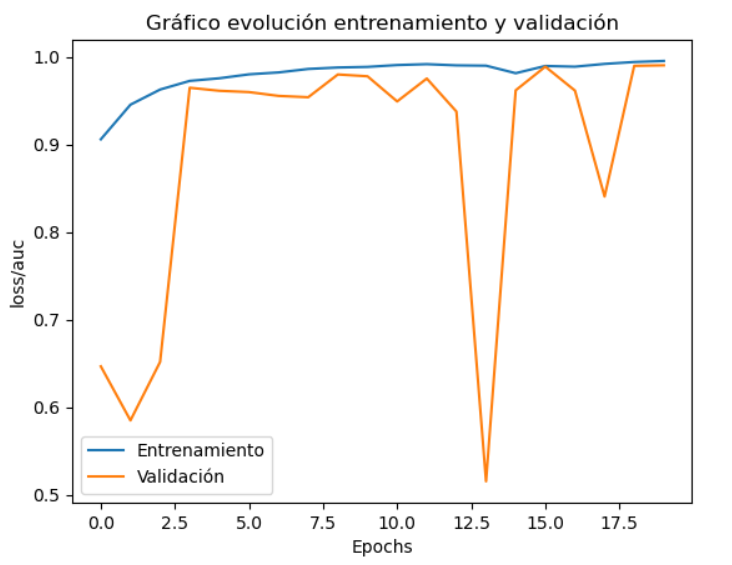
\includegraphics[width=0.80\textwidth]{img/grafica_auc_Simple3_64_100_16.PNG}
    \caption{Gráfica AUC rendimiento del entrenamiento y la validación del modelo final. Fuente propia.}
    \label{fig:grafica_auc_Simple3_64_100_16}
\end{figure}
\FloatBarrier

En la gráfica \ref{fig:grafica_auc_Simple3_64_100_16}, se visualiza el rendimiento del modelo final (``Simple3'' \textit{batch size} = 64 y 100 y 16 neuronas en las últimas capas) respecto a la métrica ``AUC'' a lo largo de tiempo tanto para el entrenamiento como la validación. Este tipo de gráficas sirven para determinar si el modelo está aprendiendo correctamente o, por el contrario, existe sobreajuste o subajuste.

Los valores de AUC obtenidos durante el entrenamiento (``auc''), miden la capacidad del modelo para distinguir entre clases en el conjunto de entrenamiento mientras que los valores de AUC obtenidos durante la validación (``val\_auc'') miden la capacidad del modelo para distinguir entre clases en el conjunto de validación. En ambos casos, un valor mayor indica un mejor modelo.

Por lo tanto, tal y como se puede apreciar en la gráfica \ref{fig:grafica_auc_Simple3_64_100_16} la línea de entrenamiento comienza en las primeras épocas con un AUC de 0,9 aproximadamente y, a medida que pasan las épocas, el AUC aumenta casi hasta 1, lo que significa que el modelo mejora su capacidad para clasificar correctamente los ejemplos en el conjunto de entrenamiento a medida que las épocas avanzan. Así mismo, la línea de validación presenta dos picos notables en la época 2 y la época 13 (aproximadamente) y un pico algo menor en la época 17 donde el AUC es menor. Esto puede deberse a un sobreajuste temporal o a unos datos empleados para la validación en esas épocas especialmente atípicos (diferentes al resto), lo que dificulta su identificación.

\begin{figure}[h]
    \centering
    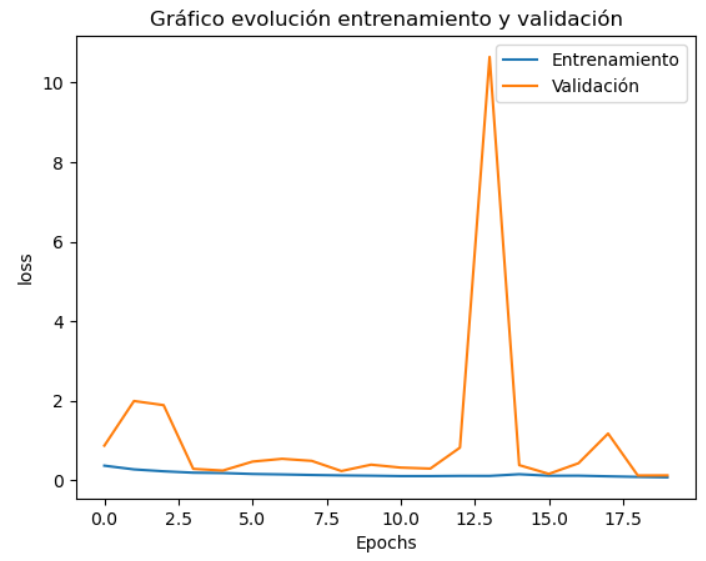
\includegraphics[width=0.80\textwidth]{img/grafica_loss_Simple3_64_100_16.PNG}
    \caption{Gráfica ``\textit{loss}'' rendimiento del entrenamiento y la validación del modelo final. Fuente propia.}
    \label{fig:grafica_loss_Simple3_64_100_16}
\end{figure}
\FloatBarrier

Por otro lado, en la gráfica \ref{fig:grafica_loss_Simple3_64_100_16}, se visualiza el rendimiento del modelo final respecto a la métrica ``\textit{loss}'' a lo largo de tiempo tanto para el entrenamiento como la validación. 

Los valores de \textit{loss} obtenidos durante el entrenamiento (``\textit{loss}''),miden el error del modelo en el conjunto de entrenamiento mientras que los valores de \textit{loss} obtenidos durante la validación (``val\_loss'') miden el error del modelo en el conjunto de validación. En ambos casos, un valor lo más cercano al 0 indica un mejor modelo.

Por lo tanto, tal y como se puede apreciar en la gráfica \ref{fig:grafica_loss_Simple3_64_100_16} la línea de entrenamiento comienza en las primeras épocas con un error (``\textit{loss}'') de 0,4 aproximadamente y, a medida que pasan las épocas, el error va disminuyendo acercándose al 0, lo que significa que el modelo está aprendiendo correctamente en el conjunto de entrenamiento. Así mismo, la línea de validación presenta un gran pico en la época 13 y dos picos menores en la época 2 y la época 17 (aproximadamente) donde el error es mayor. Esto puede deberse, de igual manera que ocurría en la gráfica referida al AUC, a un sobreajuste temporal o a unos datos empleados para la validación en esas épocas especialmente atípicos (diferentes al resto) lo que dificulta su identificación.

\section{Discusión.}

En primer lugar, hay que tener en cuenta que se trata de unos resultados obtenidos a partir de un CPU convencional en un ordenador personal. Ya que, debido a diversos problemas explicados en la sección de ``Inconvenientes'' del siguiente apartado, no se ha podido acceder a ningún supercomputador. 

Por lo tanto, estos resultados presentan algunas limitaciones. El ordenador personal no posee la misma capacidad de procesamiento y memoria que los supercomputadores por lo que, se ha tenido que reducir el número de épocas durante el entrenamiento lo que provoca unos resultados subóptimos afectando en su precisión y eficacia.

Teniendo en cuenta esto y que los resultados obtenidos no son los ideales, se trata de unos resultados razonablemente buenos ya que, tal y como se puede ver en la tabla \ref{fig:tabla_alexNet_arqu_batch} se ha alcanzado un AUC de 0,99, un error de 0,14, una exactitud de 0,95 y una precisión de 0,97. Además, en las gráficas obtenidas se puede ver cómo, a pesar de tener tres picos donde el conjunto de entrenamiento no se generalizan correctamente con el conjunto de validación, no se trata un comportamiento mantenido a lo largo de todas las épocas ya que, el modelo se corrige en las épocas posteriores.

Los tres picos obtenidos en las gráficas \ref{fig:grafica_loss_Simple3_64_100_16} y \ref{fig:grafica_auc_Simple3_64_100_16}, también pueden deberse a una poca cantidad de datos para el entrenamiento de una red neuronal ya que, otro punto a tener en cuenta es que, para un correcto entrenamiento de una red neuronal convolucional es necesario emplear grandes cantidades de datos \cite{kundu2021pneumonia} y, en este caso aun tratándose de un gran número de imágenes (5856 concretamente), en el ámbito de redes neuronales son necesarias muchas más para trabajar de forma idónea. Mas aun, teniendo en cuenta que se emplea la CNN de AlexNet donde cuanto más grande y variado sea el conjunto de datos, mejor rendimiento y generalización se obtiene del modelo.

En la matriz de confusión se observa un gran número de casos donde el modelo predice correctamente tanto los casos de neumonía (valor 818) como los casos sin ella (valor 291) y, 37 casos han sido diagnosticados como normal siendo neumonía, un valor mucho menor que el inicial.

Para concluir, se han obtenido resultados relativamente buenos teniendo en cuenta todos estos problemas, pero, aún queda mucho trabajo por hacer antes de poder introducir este tipo de IA en el ámbito clínico. Ya que, para eso es necesario contar con resultados prácticamente perfectos en todos los sentidos y, por ahora no es el caso.





